\section{Introduction}

\section{Concepts Suivis}

\subsection{Méthodologie DevOps}

\subsection{Automatisation des Tâches}

\subsection{Infrastructure as Code (IaC)}
Cette partie discute le principe d'\texttt{IaC; Infrastructure as Code}\cite[Chapter~4]{thePracticeOfSystemAndNetworkAdministration} (en français ``\texttt{Infrastructure en tant que Code}''), une stratégie d'administration des systèmes dont l'infrastructure est provisionnée et gérée à travers des fichiers de configurations programmés au lieu du travail manuel. Cette méthode nous permet de gérer nos infrastructures en utilisant les même techniques de développement des applications comme les systèmes de contrôle des versions, tests unitaires, l'Intégration Continue et le Déploiement Continue (CI/CD). 
\newline

Avec le principe d'\texttt{IaC}, on effectue les changements aux systèmes en changeant les fichiers de code et de configuration utilisés, et non directement sur ces systèmes. Le code source utilisé pour décrire notre infrastructure représente notre environnement de travail, il décrit les machines, leurs programmes et applications, les connexions réseaux entre elles ... etc. On développe notre infrastructure la façon comment un développeur produit son application.
\newline

\texttt{IaC} n'est pas un systèmes ni un langage de programmation, c'est un principe et un méchanisme à suivre et implémenter à travers les outils disponibles pour cela; Puppet\cite{puppetWiki}, Chef\cite{chefWiki}, Docker (voir section \ref{docker}) ... etc.

\subsubsection{Avantages d'Infratructure as Code}

Par l'adoption de cette stratégie, on bénificie de trois avantages majeures :
\begin{itemize}
  \item\textbf{\emph{Coût réduit}} : Tout simplement parce que le travail manuel est presque éliminé. L'automatisation permet qu'une personne réalise les tâches de plusieurs, ce qui veut dire moins de personnes employées!
  \item\textbf{\emph{Déploiement rapide}} : Les tâches sont exécutés de manière rapide et en parallèle. 
  \item\textbf{\emph{Moins de risque}} : Moins de risque d'erreurs et bugs en suivant les techniques de développement informatique. Aussi, moins de risque de sécurité avec les différents types de tests automatisés.
\end{itemize}

\subsubsection{Principes d'Infratructure as Code}

Les principes d'\texttt{IaC} sont les suivants :
\begin{itemize}
  \item\textbf{\emph{Tous les changements à travers les fichiers source de configuration}} : Ne pas se connecter aux serveurs pour effectuer les changements, il vaut mieux utiliser les fichiers du code et de configuration.
  \item\textbf{\emph{La documentation à travers le code source}} : Les fichiers de documentation et ses illustrations doivent être générés à partir du code et des fichiers de configuration parce qu'ils sont la source fiable d'architecture de l'infrastructure.
  \item\textbf{\emph{Utilisation d'un système de contrôle des versions}} : Tous les fichiers du code et de configuration doivent être contrôlés par un système de contrôle des versions pour garder l'historique des changements.
  \item\textbf{\emph{Implémentation de l'Intégration / Déploiement Continue (CI/CD)}} : Exécutez les tests et le processus d'automatisation après chaque modification pour identifier les erreurs rapidement puis les corriger. 
  \item\textbf{\emph{Un petit changement à la fois}} : Les erreurs sont simples à trouver lorsqu'elles résident dans un petit changement des fichiers. De même, les petits changements sont plus simple à déploier et/ou annuler que les grands changements.
  \item\textbf{\emph{Le service est toujours disponible}} : Il vaut mieux appliquer des techniques pour garder le service offert disponible aux moments des mises à jour (exemples: la haute disponibilité, la tolérance aux pannes ...). Comme ça on peut effectuer des changement plus fréquemment sinon il sera difficile d'applique le principe précédent!
\end{itemize}

\subsection{Continuous Integration / Deployment (CI/CD)}

\subsubsection{Continuous Integration (CI)}

\subsubsection{Continuous Deployment (CD)}

\section{Technologies Utilisées}

\subsection{GitLab} \label{gitlab}

Pour les développeurs en particulier, et chaque utilisateur informatique en général, garder la trace des changements effectués sur les fichiers est une fonctionnalité essentielle pour une bonne gestion du code source. La possiblité d’annuler les changements, retourner à une version antérieure d’un fichier, comparer les modifications entre les versions … et plus de fonctionnalités sont les objectifs d’un système de gestion des versions. 
\newline

SVN et Git sont deux exemples des systèmes de contrôle de version open source, avec Git le plus populaire aujourd'hui.

\subsubsection{Git : Gestion des Versions Décentralisé}
Git est un système distribué de contrôle des versions libre et open source, créé en 2005 par Linus Torvalds, fondateur du noyau Linux. Au moment d’écriture de ces lignes, git a arrivé à sa version 2.13. 
\newline

Git offre “toutes” les fonctionnalités fournies par les concurrents du marché, avec l’avantage de la décentralisation, ce qui permet d’utiliser Git de manière similaire en local comme en équipe dans le réseau.
\newline

\textbf{Systèmes de Contrôle des Versions Locaux} \newline
Dans un premier temps, l’approche adopté par les utilisateurs était la copie des fichiers dans un dossier. Cet approche n’était pas efficace car il était souvent sujet à l’erreur si par exemple vous oubliez le dossier sur lequel vous êtes et vous écrasez le – ou les – fichier erroné!


\begin{figure}[H]
    \centering
    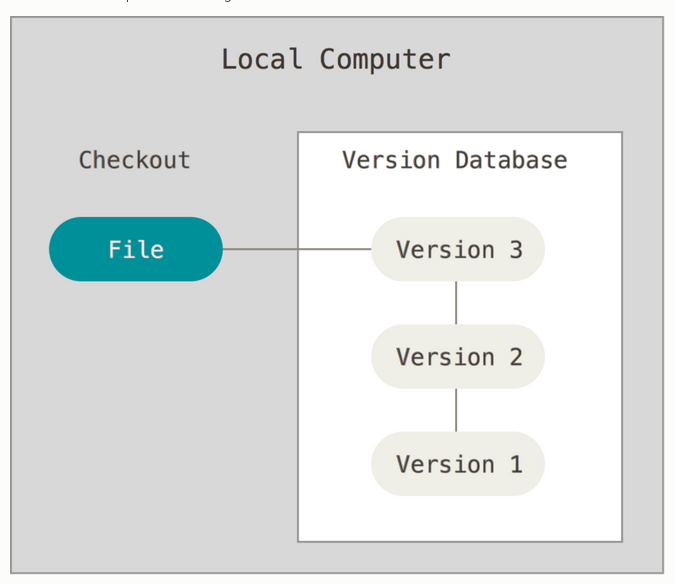
\includegraphics[width=9cm]{images/local-scm.png}
    \caption{Principe d'un système de contrôle des versions local.}
    \label{fig:local-scm}
\end{figure}

Pour éviter ces accidents, les développeurs ont créé des systèmes de contrôle des versions locaux qui avaient des bases de données qui stockent les changements des fichiers. Le plus populaire de ces systèmes était RCS, qui travaille avec le principe de stocker les différences entre les fichiers – appelées patches - sur le disque sous un format spécial de telle manière qu’il soit capable de restorer le contenu de n’importe quel fichier dans n’importe quel moment en se basant sur les patches.
\newline

\textbf{Systèmes de Contrôle des Versions Centralisés} \newline
Les développeurs avaient besoin de collaborer entre eux mais sur plusieurs systèmes. Pour attaquer ce besoin, les systèmes de contrôle des versions centralisés ont été créés. Ces systèmes comme CVS et SVN ont un seul serveur qui contient toutes les versions des fichiers du code source et un nombre de clients qui copie les fichiers depuis ce serveur central. Cela était le standard pendant plusieurs années.

\begin{figure}[H]
    \centering
    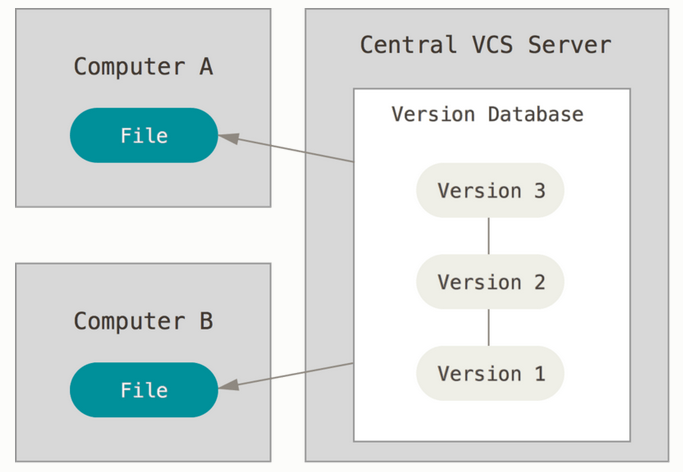
\includegraphics[width=12cm]{images/central-scm.png}
    \caption{Principe d'un système de contrôle des versions central.}
    \label{fig:central-scm}
\end{figure}

Le point faible majeur de cet approche était le point de défaillance unique; un seul serveur contient tous les fichiers. Si ce serveur tombre en panne, personne ne peut collaborer ou effectuer des échanges avec lui, il y avait même le risque de tout perdre si le support de stockage tombe en panne et pas de backup était effectué. Ces incovénients ont été addressés par les systèmes décentralisés.
\newline

\textbf{Systèmes de Contrôle des Versions Décentralisés} \newline
Au lieu de cloner seulement quelques fichiers depuis le répertoire central, les systèmes de contrôle des versions décentralisés permettent le clonage complet du répertoire, effectuer les changements, et puis pousser le répertoire entier au serveur central à nouveau. Si le serveur central tombe en panne, n’importe quel répertoire chez les utilisateurs peut être copié au nouveau serveur, et continuer la collaboration comme avant. En principe, chaque clone du répertoire central par les utilisateurs est considéré comme un backup complet de ce répertoire!

\begin{figure}[H]
    \centering
    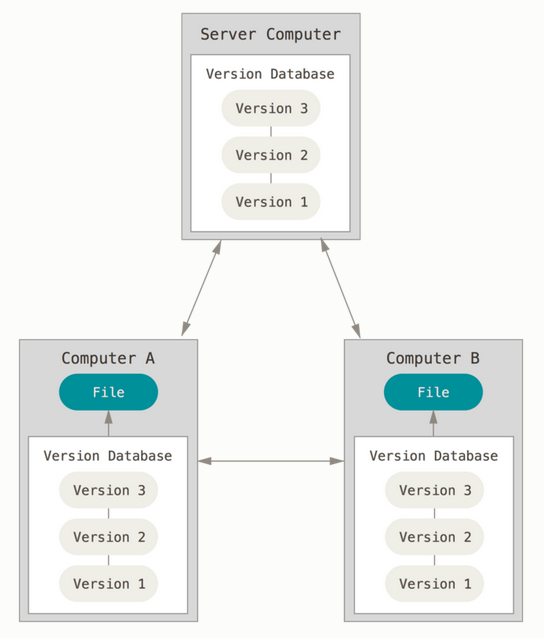
\includegraphics[width=9cm]{images/distributed-scm.png}
    \caption{Principe d'un système de contrôle des versions distribué.}
    \label{fig:distributed-scm}
\end{figure}

Git et Mercurial sont parmi les systèmes décentralisés les plus populaires, avec Git en top pour sa richesse en termes de fonctionnalité et comme étant un projet libre et open source supporté par une grande communauté et utilisé par les tops entreprises de technologies mondiales.

\subsubsection{C’est quoi GitLab?}
Git est un logiciel basé sur la ligne de commandes, mais pas tout le monde travaille avec elle. Avec les environnements de développement intégrés – IDEs – et les frameworks, les développeurs – et autres – souvent utilisent les interfaces graphiques pour ses tâches quotidiennes, ce qui impose d’avoir des outils graphiques pour Git.
\newline

Alors GitLab est une application web pour la gestion des répertoires Git créée en 2011, similaire à GitHub, développée en langages Ruby et Go. La société GitLab Inc. fournit GitLab en deux produits; une version Communautaire avec une licence open source, et une version Commerciale avec plus de fonctionnalités destinées aux grandes Entreprises.

\begin{figure}[H]
    \centering
    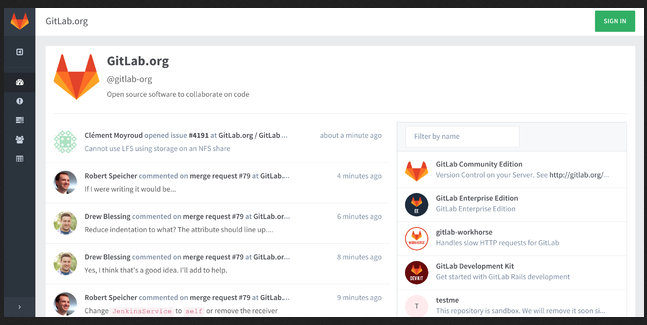
\includegraphics{images/exemple-gitlab.png}
    \caption{Une interface web sur GitLab.}
    \label{fig:exemple}
\end{figure}

On peut dire que GitLab permet d’avoir notre propre GitHub local. GitLab fournit toutes les fonctionnalités de base de Git, et bien d’autres comme les pipelines l’Intégration/Déploiement Continue , un Wiki intégré, gestion des utilisateurs et groupes d’utilisateurs, nombre de répertoires Git privés et/ou publics illimités, la trace et gestion des problèmes – appelés Issues – et des “A Faire” - appelés Todos - , les notifications , … et autres.
\newline

FY Computing accueille des dizaines de développeurs, webdesigners et sysadmins et veut bénéficier des services comme ceux de GitHub mais hébérgé en local et illimités, alors GitLab était notre choix unique pour cela. Alors on a procédé à hébergé l’application web GitLab à l’aide des Conteneurs Docker.

\newpage

\subsection{Ansible} \label{ansible}

\newpage

\subsection{Docker} \label{docker}
Docker est un logiciel open source qui automatise le déploiement d'applications dans des Conteneurs logiciels. Ceci permet d'étendre la flexibilité et la portabilité d’exécution d'une application, que ce soit sur la machine locale, un cloud privé ou public, une machine nue, etc. 
\newline

Docker étend le format de conteneur Linux standard (LXC) avec une API de haut niveau fournissant une solution de virtualisation qui exécute les processus de façon isolée. Docker utilise LXC, cgroups, et le noyau Linux lui-même. Contrairement aux machines virtuelles traditionnelles, un conteneur Docker n'inclut pas de système d'exploitation,  mais s'appuyant sur les fonctionnalités du système d’exploitation fournies par l'infrastructure sous-jacente.

\subsubsection{Conteneurs vs Machines Virtuelles}
En principe, les Conteneurs sont l'encapsulation d'une application avec ses dépendences. En premier temps, ils apparaissent comme une forme légère des VMs (i.e. Machines Virtuelles). Les deux techniques contiennent un système d'exploitation isolé surlequel on peut déployer nos applications. Cependant, les Conteneurs apportent de nombreux avantages difficiles (voir impossible!) d'avoir avec les VMs :
\begin{itemize}
\item Les Conteneurs partagent les ressources avec le système hôte beaucoup plus efficace que les VMs. 
\item Les Conteneurs peuvent être lancer et arrêter dans des millisecondes. 
La portabilité des Conteneurs élimine le guerre des dépendances inter-systèmes, garantie que ça va marcher indépendamment du système hôte. 
\item Les Conteneurs sont incroyabelement légers permettant aux utilisateurs d'exécuter des dizaines (même plus) de Conteneurs en même temps pour simuler un vrai environnement de production distribué, ce qui n'est pas le cas souvent avec les VMs. 
\item Les clients finaux des applications peuvent télécharger puis exécuter ses applications complexes rapidement sans devoir passer des heures de souffrance des installations et de configurations. 
\newline
\end{itemize}

De plus, l'objectif essentiel d'un Conteneur est de rendre une application complètement portable et autonome, au contraire des VMs qui visent la virtualisation totale d'un environnement externe.

\begin{figure}[H]
    \centering
    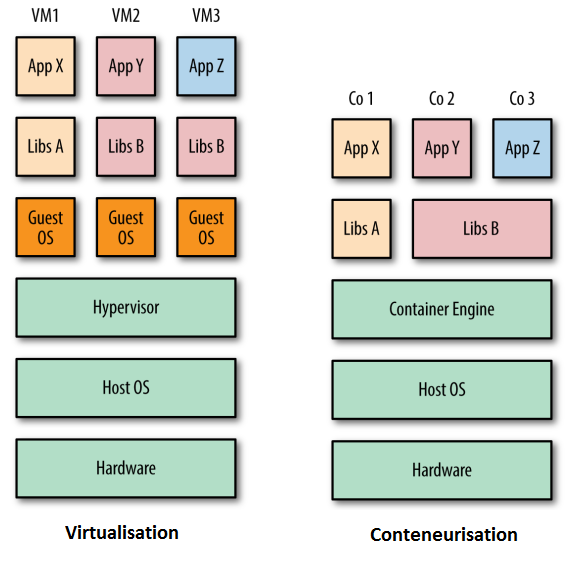
\includegraphics[width=12cm]{images/vm-vs-container.png}
    \caption{Exemple de trois applications X, Y et Z déployées à gauche à l'aide des VMs et à droite en utilisant des Conteneurs.}
    \label{fig:vm-vs-container}
\end{figure}

\subsubsection{Introduction à Docker}

En réalité, la Conteneurisation existe depuis longtemps sur les systèmes UNIX/Linux sous plusieurs formes ; chroot, jail. Après la création de la technologies open source de conteneurisation OpenVZ (anciennement Virtuozzo) par Parallels Inc. et LXC (Linux Containers) par Google .. et autres, Docker a apporté la pièce manquante de la solution mature et complète en 2013.
\renewcommand{\appendixtocname}{Annexes}

Docker fournit un ensemble de produits et services à savoir :
\begin{itemize}
\item \textbf{Docker Engine} est le moteur de Conteneurisation qui fournit une interface d'execution des Conteneurs simple et efficace. 
\item \textbf{Docker Hub} est un espace Cloud public qui contient des centaines des images Docker créées par la communaté pour partager et commencer rapidement à partir de ce qu'existe déjà. 
\item \textbf{Docker Store} est similaire à Docker Hub mais fournit des Images certifiées  pour les Entreprises (parfois payantes). 
\item \textbf{Docker Swarm}, un gestionnaire des clusters de Conteneurs. 
\end{itemize}

Après l'adoption rapide de la technologie des Conteneurs à l'aide de Docker, ce dernier a devenu le standard dans l'industrie, ce qui a mené à créer l'ogranisation Open Container Initiative par Docker, Google, Microsoft, CoreOS et autres pour normaliser le standard.
\newline

\subsubsection{Principes Docker}

\begin{figure}[H]
    \centering
    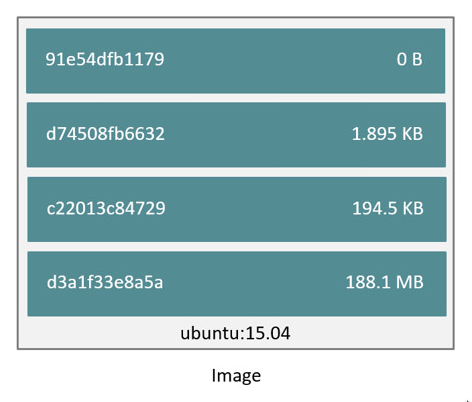
\includegraphics[width=10cm]{images/ubuntu-image.png}
    \caption{Les couches de système de fichiers d'une Image Docker Ubuntu.}
    \label{fig:ubuntu-image}
\end{figure}

Le fonctionnement Docker se base sur les principe des `Images Docker`. Une Image Docker est la base des Conteneurs Docker. Une Image Docker est une collection ordonnée des changements effectués sur un système de fichiers et de ses paramètres d’exécutions, pour l’utilisation dans un Conteneur en cours d’exécution. Généralement, une Image est l’union des couches – en lecture seule - des systèmes de fichiers stockées l’une au-dessus de l’autre pour former le système de fichiers racine d’un Conteneur. Chacune de des couches est identifiée par un code de hashage unique généré par Docker au moment de construction de l’Image. Les Images Docker n’ont aucun état et ne changent jamais.
\newline

Une Image est construite automatiquement par Docker à partir d’un fichier texte appelé Dockerfile, qui contient un ensemble d’instructions et commandes,  ordonnées, pour construire une telle Image. Dockerfile a un format specifique et accèpte un ensemble d’instructions spécifiques qui définissent le contenu des couches de systèmes de fichiers de l’Image finale. Une Image bien construite est celle qui est légère au maximum possible en contenant seulement les applications nécessaires au fonctionnement du service fournit et le stricte minimum des couches de systèmes de fichiers.
\newline

Pour éviter la répétition, Docker fournit un espace de stockage dans le Cloud gratuit pour partager les Images Docker avec Docker Hub. Récemment, Docker a annoncé son service Cloud payant Docker Store riche en fonctionnalités avancées et destiné aux Entreprises. Ceci permet de démarrer rapidement avec Docker en exploitant des centaines d’Images publiques, sans perdre le temps pour créer ce que les autres l’ont déjà fait!
\newline

Chaque Image Docker est identifié soit par un nom unique – appelé Tag - sous le format “<repertoire>/<service>:<version>” qu’on peut l’y affecter, ou par un code de hashage généré automatiquement par Docker. Le Tag est souvent utilisé dans la gestion des Images clairement pour sa simplicité à retenir. 
\newline

\begin{figure}[H]
    \centering
    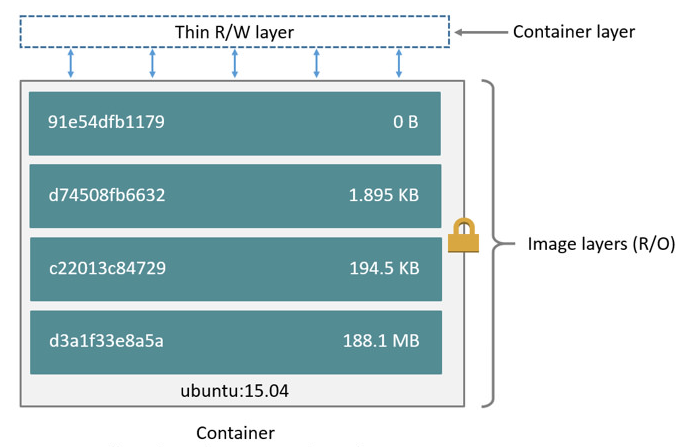
\includegraphics[width=12cm]{images/ubuntu-container.png}
    \caption{Un Conteneur Docker basé sur l'Image Docker d'Ubuntu.}
    \label{fig:ubuntu-container}
\end{figure}

Dans l’autre côté, un Conteneur Docker est tout simplement l’instance active – avec état - en cours d’exécution d’une Image Docker. C’est similaire au principe des Classes et ses Objets dans la programmation orientée Objets. l’exécution d’un Conteneur Docker signifie la création d’une couche légère et écrivable du système de fichiers – au-dessus des couches enregistrées de l’Image source -, dans laquelle toutes les modification effectuees pendant l’exécution du Conteneur seront sauvegardées, jusqu’à la destruction de ce Conteneur. Cette structure permet à plusieurs Conteneurs de partager la même Image, même plusieurs Images de partager les couches identiques.
\newline

\subsection{JavaScript MEAN Stack}

Lorsqu'on dit "développement Full Stack", on parle du développement de toutes les parties d'un site ou application web, depuis la conception de la base de données et programmation du serveur web dans le Back End jusqu'à l'interface graphique des utilisateurs dans le Front End.
\newline

Le MEAN\cite{gettingMEAN} Stack se compose de 4 technologies principales :
\begin{itemize}
\item \textbf{M}ongoDB - La base de donnees.
\item \textbf{E}xpressJS - Framework de développement Web (Back End).
\item \textbf{A}ngularJS - Framework de développement Web (Front End).
\item \textbf{N}odeJS - Serveur Web.
\newline
\end{itemize}


MongoDB a été créé en 2007 et maintenu par MongoDB Inc., il était anciennement connu sous le nom 10gen.
\newline

ExpressJS est un projet open-source lancé en 2009 par T.J. Holowaychuck et considéré le framework web le plus populaire pour NodeJS.
\newline

AngularJS aussi un projet open-source supporté par Google, il est au marché depuis 2010 et très active en terme de développement et d'innovation.
\newline

NodeJS a été créé en 2009 et se base sur le moteur open-source de JavaScript V8 développé par Google.

\subsubsection{MongoDB}

La persistence des données est une phase indispensable dans le cycle de vie d'une application. Le choix de la base de données dans le MEAN Stack est tombé sur MongoDB, le 'M' dans ``MEAN''. En général, on est habitué au concept des lignes et colonnes dans les bases de données relationnelles, mais MongoDB n'est pas comme ça! MongoDB est un serveur open-source de bases de données orienté document\cite{documentDB} qui est très performant et évolutif.
\newline

Les \texttt{Documents} de MongoDB sont similaires aux objects \texttt{JSON - JavaScript Object Notation}\cite{json}, avec les valeurs des champs peuvent inclure d'autre documents, des tableaux, et des tableaux de documents. Les Documents - aussi connu sous le nom Objets - correspondent à des types de données natives dans plusieurs langages de programmation (comme JavaScript)ce qui reflète un point fort de ce type des bases de données. De plus, les Documents embarqués et les tableaux des Documents réduit le besoin d'effectuer des jointures coûteuses en terme de performance. MongoDB supporte les données semi-structurées, alors il offre de la polymorphisme à travers ses schémas de données dynamiques. Par contre, MongoDB n'est pas une base de données transactionnelle, et ne doit pas être utilisé pour cela\cite{mongoDBAndMySQLCompared}.
\newline

Mongoose est un module de modélisation des objets MongoDB pour NodeJS. Souvent les applications nécessite une modélisation de ces structures de données (et pas la base de données MongoDB elle-même!), donc Mongoose permet la définition d'un schéma de donnée dont on définit quel type de données peut être dans un Document, ou bien quelle donnée doit être dans ce Document ... etc. Plus que la modélisation, Mongoose fournit une toute couche entière de fonctionnalités au dessus de MongoDB, très utiles dans le développement des applications Web (Gestion des connexions à MongoDB, validation des données, lecture et écriture simple de Documents ... etc).\cite{mongooseDocs}

\subsubsection{ExpressJS}

Dans la création des serveurs et applications Web, il y a des tâches commune qui se répètent et on doit les faire à chaque fois. Express est un framework Web pour NodeJS créé pour ce genre de tâches. Sachant que NodeJS est un plateforme et non pas un serveur, Il nous donne la possibilité d'être créative dans la création de notre serveur Web mais un peu difficile pour développer un serveur Web simple. 
\newline

Express adresse cette difficulté en ajoutant une couche d'abstraction au-dessus de NodeJS pour créer un serveur Web qui écoute pour les requêtes et retourne les réponses adéquates. Parmi les avantages d'Express est sont API de routage Web, qui fournit une interface simple pour lier des addresses URL vers un morceau du code source qui peut soit retourner une page HTML, lire depuis une base de données, écrire dans la base de données ... etc. Ceci rend la taĉhe de créer cette même fonctionnalité avec NodeJS beaucoup plus rapide, simple et facile à maintenir.

\subsubsection{AngularJS}

En résumé, AngularJS est un framework JavaScript pour travailler avec les données directement dans le côté Client (i.e. Front End) et basé sur l'architecture \texttt{MVC}\cite{mvcArchitecture}. On peut développer une application Web complète juste avec les autres trois technologies MEAN, mais AngularJS nous permet de déplacer peu des traitements de données dans le côté Serveur vers le côté Client, souvent en laissant le programme du Serveur traite la communication avec la base de données.
\newline

AngularJS se base sur la liaison bidirectionnelle de données (en anglais \texttt{Two-Way Data Binding}) à l'opposée de la liaison unidirectionnelle de données qui est la méthode traditionnelle. Cette dernière est utilisée déjà lorsqu'on développe un projet avec MongoDB, NodeJS et Express seulement; NodeJS récupère les données depuis MongoDB puis Express utilise des modèles (en anglais \texttt{Templates}) pour compiler ces données en HTML délivré par la suite au Client [voir la figure \ref{fig:one-way-data-binding}]. Dans ce genre de liaison, la majorité du travail est effectué dans le côté Serveur. 

\begin{figure}[H]
    \centering
    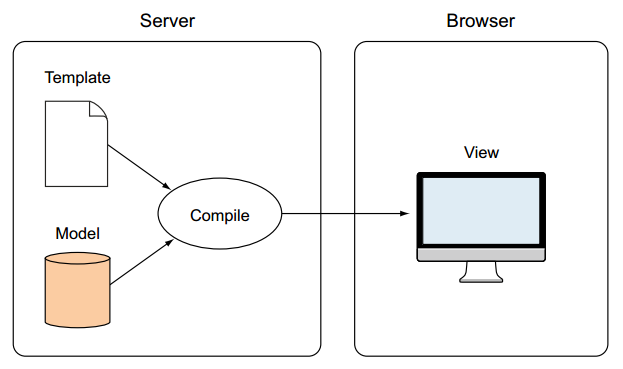
\includegraphics[width=10cm]{images/one-way-data-binding.png}
    \caption{Liaison unidirectionnelle de données dans le côté Serveur.}
    \label{fig:one-way-data-binding}
\end{figure}

Par contre, la liaison bidirectionnelle des données est différente. \texttt{Template} et les données sont envoyées séparémment au client Web. Le client Web est maintenant responsable de compiler le \texttt{Template} en une vue HTML et les données en \texttt{Model}. La différence majeure est que la Vue est ``vivante'', cest-à-dire si le \texttt{Model} change, la \texttt{View} reflète ce changement instantanémment, et vice-versa [voir la figure \ref{fig:two-way-data-binding}].

\begin{figure}[H]
    \centering
    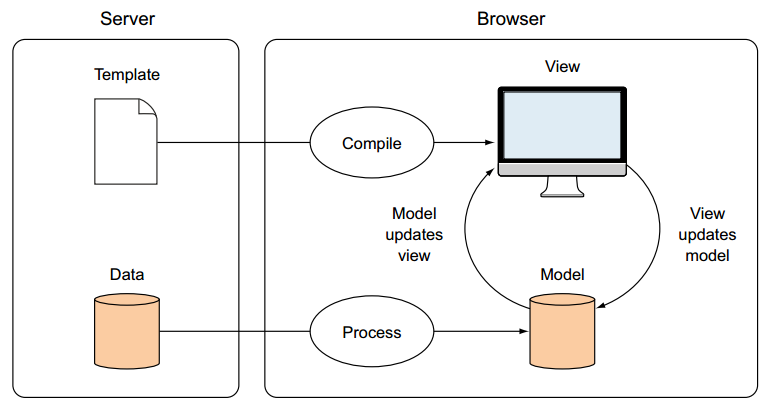
\includegraphics[width=11cm]{images/two-way-data-binding.png}
    \caption{Liaison bidirectionnelle de données avec AngularJS dans le côté Client.}
    \label{fig:two-way-data-binding}
\end{figure}

\subsubsection{NodeJS}

NodeJS est la fondation du MEAN Stack. NodeJS est un environnement JavaScript de côté serveur qui est évènnementiel avec des requêtes d'entrée et de sortie non-bloquantes et basé sur le moteur JavaScript V8 de Google. En résumé, NodeJS nous permet de créer notre serveur Web avec nos applications web en top. Il n'est pas un langage ni un serveur Web lui-même, mais contient une bibliothèque de serveur HTTP, ce qui veut dire qu'on n'aura pas besoin d'avoir un serveur Web externe (Apache, Internet Information Services ``IIS'' ...) pour exécuter nos projets Web. Malgré que ceci nous donne un contrôle étendu sur la façon comment notre serveur Web fonctionne, mais il complique la tâche de sa création et son lancement rapide.
\newline

Un serveur Web créé par NodeJS est \texttt{``single-threaded''}, cest-à-dire tous les clients seront servi par un seul thread, le même thread. Cet approche est différent aux autres serveurs Web qui sont considérés \texttt{``multithreaded''} (comme Apache) qui affectent un thread pour chaque connexion d'un client. De plus, les évènnement d'entrée et de sortie pour NodeJS sont non-bloquants\cite{blockingVSnonBlocking}, ce qui permet à l'application web de ne pas se bloquer en attente des résponses aux requettes vers les ressources sur le système, et cela permet à NodeJS d'être beaucoup plus rapide\cite{nodeJSvsPHP}.
\newline

NPM est un gestionneur des modules installé avec NodeJS. Il nous donne la possibilité de télécharger des modules NodeJS pour étendre les fonctionnalités de nos applications. Au moment de la rédaction, NPM héberge presque demi-million de modules gratuitement ce qui montre combien de fonctionnalités prêtes à utiliser qui peuvent être ajoutées à nos applications NodeJS.

\section{Conclusion}
